\chapter[Paper: A Bayesian approach to modeling lost person behaviors based on terrain features in Wilderness Search and Rescue]{Paper: A Bayesian approach to modeling lost person behaviors based on terrain features in Wilderness Search and Rescue\footnote {Published in CMOT 2010 (Computational and Mathematical Organization Theory) journal. Authors are Lanny Lin, and Michael A. Goodrich.}}
\label{chap:CMOT2010}

\begin{abstract}
In Wilderness Search and Rescue (WiSAR), the Incident Commander (IC) creates a probability distribution map of the likely location of the missing person. This map is important because it guides the IC in allocating search resources and coordinating efforts, but it often depends almost exclusively on prior experience, subjective judgment, and a missing-person profile,. We propose a Bayesian model that uses publicly available terrain features data to help model lost-person behaviors. This approach enables domain experts to encode uncertainty in their prior estimations and also makes it possible to incorporate human behavior data collected in the form of posterior distributions. These distributions are used to build a first-order Markov transition matrix for generating a temporal, posterior predictive probability distribution map. The map can then be augmented as desired by search and rescue workers to incorporate additional information. Using a Bayesian $\chi^2$ test for goodness-of-fit, we show that the model fits a synthetic dataset well. This model also serves as a foundation for a larger framework that allows for easy expansion to incorporate additional factors, such as season and weather conditions, that affect the lost-person's behaviors.
\end{abstract}

%=====================================================================================================
\section{Introduction}
\label{3intro}

In the priority search phase\footnote{Four qualitatively different types of search strategies are used in WiSAR: hasty search, constraining search, priority search, and exhaustive search. See~\cite{Goodrich2008Supporting} for more details.} of Wilderness Search and Rescue (WiSAR), a probability distribution map for the likely place to find the missing person is created using terrain features, a profile of the missing person, weather conditions and subjective judgment of expert searchers (see~\cite{Koester2008Lost}). The Incident Commander (IC) uses this map to allocate resources, to direct the search, and to coordinate rescue workers. Search and rescue resources are typically limited, meaning only a small portion of the area can be covered in the first few hours of the search. However,~\cite{Setnicka1980Wilderness} and \cite{Syrotuck2000Introduction} show that as time progresses, the survivability of the missing person decreases and the effective search radius increases by approximately 3km/hour. Therefore, areas with high probabilities are searched first in hope of finding the missing person quickly. The probability distribution map created by the IC can also be used by manned or unmanned aerial vehicles for path planning purposes, thus facilitating effective aerial search. The quality of the probability distribution map is critical to the WiSAR operations and can mean the difference between life and death for the missing person.

We propose a Bayesian approach in modeling lost-person behaviors to generate such a probability distribution map automatically. The search and rescue workers can then augment this base map to incorporate their own beliefs to generate the final probability distribution map. We argue that using the Bayesian approach to automatically generate the map can be beneficial in the following ways: 

1) The Bayesian approach easily allows the inclusion of prior data (in the form of subjective judgment of the SAR volunteers), the profile (travel direction and dispersion characteristics) of the missing person, etc.

2) This approach allows the search and rescue workers to naturally incorporate their uncertainty by specifying a mean and a variance, which we will then incorporate into a Beta distribution to facilitate a robust Bayesian model.

3) This approach allows the incorporation of actual human behavior data collected to generate posterior beliefs.

4) The map generated using the Bayesian model means that the search and rescue workers do not have to build the probability distribution map from scratch and it reduces the chance that the search and rescue workers might overlook a certain area that should have been allocated higher probability.

5) The probability distribution map can be dynamically updated as time progresses. Assuming a first-order Markov process, the Bayesian model can easily incorporate the time element and thereby allow the search and rescue workers to observe how the proposed probability distribution map changes over time, especially as information is collected. Such capability can be useful if the search and rescue operation takes an extended period of time.

Many factors affect how the probability distribution map might turn out. Examples include the season of the year, the weather conditions, the profile of the missing person (age, gender, professions, intention, etc., which translate into direction, distance, and dispersion of travel), and the terrain features of the area. The Bayesian model proposed here mainly focuses on the terrain features, specifically, the topography type, vegetation coverage, and local slope. However, the model is designed so that it can be easily extended to take other factors into consideration.

The proposed Bayesian model has the following components: The search area is first discretized into a honeycomb pattern hexagonal tessellation where each cell represents a state with topography type, vegetation type, and elevation information, which are treated independently. Local slope can then be calculated using elevation differences between the current cell and its neighbors. Expert opinions in human behaviors, experience in past search and rescue incidents, and past statistical data are incorporated to specify the terrain feature transition probability from one topography type (or vegetation or slope, respectively) to another in the form of a mean and a variance. Using samples generated from such priors, a state transition matrix is built to specify the transition probabilities from each state to all other states, which can be used to generate the prior predictive probability distribution map for any given number of time steps. Data in the form of GPS track logs\footnote{A GPS (Global Positioning System) tracking unit can log the position of the device at regular intervals with time stamps. The sequence of these position points make up a GPS track log.} are then incorporated into the model as observations so posterior beliefs can be calculated. Using the posterior beliefs, a new state transition matrix is built and used to generate the posterior predictive probability distribution map for any given number of time steps.

The rest of paper is organized as follows: In Section 2 we discuss related work. We describe the proposed model in detail in Section 3 and analyze the experiment results in Section 4. In Section 5 we evaluate the model using the Bayesian $\chi^2$ test for goodness-of-fit by~\cite{Johnson2004Bayesian}. Section 6 presents conclusions and future work.

%=====================================================================================================
\section{Related Work}
\label{sec:2}

Many search and rescue researchers have worked on analyzing historical search and rescue cases and have tried to understand and explain missing person behaviors. ~\cite{Setnicka1980Wilderness} re-told accounts of various rescue situations by the authors and others to describe wilderness search and rescue techniques and lost-person behaviors. ~\cite{Hill1998Lost} discusses a number of reorientation strategies such as random traveling, direction traveling, route sampling, direction sampling, backtracking, using folk wisdom, and staying put. ~\cite{Syrotuck2000Introduction} describes how to use mathematical models to calculate the probability of detection, probability of area and probability of success. He also describes an example search mission. In~\cite{Syrotuck2000Analysis}, he also presents a series of case studies. ~\cite{Heth1998Characteristics} tabulate crow's-flight distance traveled and dispersion of travel by different categories of wilderness users using data from between 1987 and 1996 for 162 lost-person incidents near Peter Lougheed Provincial Park in Alberta, Canada. \cite{Koester2008Lost} described the International Search \& Rescue Incident Database (ISRID), which contains 50,692 SAR incidents at the time the book was written. Chapter 8 of the book presents important statistical content of lost person behavior by subject categories. Conclusions drawn from these publications are good resources for specifying priors with our proposed model.

As more geographical information is available to the public via the Internet, researchers have begun looking at systematically utilizing such information for search and rescue applications. ~\cite{Ferguson2008GIS} discusses the application of GIS (Geographic Information System) to manage the search for a missing autistic youth in the Dolly Sods Wilderness area of West Virginia. GIS provides a platform to integrate data from various sources, allowing the search to be segmented into probability regions based on statistical analysis and a behavioral profile of the missing subject. ~\cite{Soylemez2006Utility} present a case study about a plane crash near Kutahya, Turkey and demonstrate how probability distribution maps can be generated that shrink the incident area and enable the search team to reach the area in an optimal way. Both papers show great examples of how to use GIS information to build probability distribution maps that can be used to facilitate search and rescue operations. However, they do not allow the experts to specify their uncertainty and also do not incorporate existing human behavior data into the model in a meaningful way.

Once the probability distribution map is generated, computer algorithms can take advantage of it to perform path planning for Unmanned Aerial Vehicles (UAV). ~\cite{Goodrich2008Supporting} present field reports on how UAV technology can be integrated into existing WiSAR teams. In~\cite{Bourgault2006Optimal} and a series of related papers, Bourgault et al.\ describe how to use a Bayesian model to create paths for one or multiple coordinated UAVs to maximize the amount of probability accumulated by the UAV sensors. ~\cite{Bourgault2008AugmentedNodes} also include scalable collaborative human systems in the loop and generated paths for human operators. ~\cite{Lin2009UAV} present a series of path-planning algorithms for a UAV used in WiSAR operations, which yield high-quality solutions that approximate an optimal path using a given probability distribution map.

Bayesian modeling has been used in many aspects of human behavior modeling. \cite{Tenenbaum1999Bayesian} proposes a Bayesian model for human concept learning that gives precise fits to human behavior data. \cite{Gorman2006Bayesian} present a Bayesian-based approach to extract a human player's strategic behavior and movement patterns in interactive computer games. \cite{Oliver2000Bayesian} describes a Bayesian computer vision system for modeling and recognizing human interactions in a visual surveillance task. \cite{Sanborn2008Markov} describe a method that uses correspondence between a model of human choice and the choices made by the Markov chain Monte Carlo (MCMC) algorithm.

%=====================================================================================================
\section{Terrain-Based Bayesian Model}
\label{sec:3}

In this section we describe the proposed Bayesian model in detail. First we present an overview of the model and explain how Bayes' Theorem is used to update beliefs.

%---------------------------------------------------
\subsection{Model Overview}
\label{sec:3.1}

The Bayesian model has two distinctive parts. The first part uses previously collected human behavior data (observations of how people actually traveled in various terrains) to update prior beliefs on how the lost person would transition between different terrain features. The update is achieved using the Gibbs Sampling and Metropolis-Hastings flavor of the MCMC class of algorithms shown in~\cite{Gelman2004Bayesian}. The second part then uses posterior beliefs (updated beliefs from first part) to construct a state transition matrix based on the terrain features of the search area. Using a generative approach and assuming a first-order Markov process, we can predict how the lost person might have traveled from the point last seen as time progresses.

In the first part of the model, we ask domain experts to specify the probability that the lost person would travel from one terrain feature to another. The probability is a continuous distribution and we only ask for transitional probabilities within the same category of terrain features. Therefore, specifying the probability of traveling from topography feature ``plain'' to topography feature ``hill'' would make sense while from topography feature ``plain'' to vegetation density feature ``sparse'' would not.

We use $\theta_i$ to denote each probability distribution specified by domain experts, meaning each $\theta_i$ is a prior belief and a parameter in the model. $\underline{\theta}$ represents a vector containing all the parameters of the model. We also use $\underline{F}$ to denote the set of terrain features for the search area. Following standard Bayesian notations, we use $\pi(\underline{\theta})$ to denote the joint prior belief of the entire parameter space, and $f(z|\underline{\theta}, \underline{F})$ to denote the likelihood that the lost person traveled toward various directions given the terrain feature based transitional probabilities and the known terrain features. If we already have multiple observations of what directions a lost person traveled given various terrain features, by applying Bayes' Theorem, we can write the posterior beliefs of our parameters:
\begin{align}
\label{BayesTherom}
\pi(\underline{\theta}|\underline{z})=\frac{f(\underline{z}|\underline{\theta})\pi(\underline{\theta})}{\displaystyle\displaystyle\int^{1}_{0} f(\underline{z}|\underline{\theta})\pi(\underline{\theta})d\underline{\theta}}
\end{align}
where $\underline{z}$ is a vector containing multiple observations. Here we can drop $\underline{F}$ from our equation because $\underline{F}$ is known.

In the second part of the model, since we already have the posterior beliefs (in continuous form) of how the lost person would transition from one terrain feature to another, we can sample from the posterior beliefs and then construct a state transition matrix based on the terrain features of the search area. Each state is a cell in a hexagonal tessellation, and each row of the state transition matrix consists of the transitional probabilities of traveling from one cell to every cell in the tessellation (including itself). Therefore, the state transition matrix is an $n \times n$ matrix where $n$ is the total number of cells in the tessellation, or the total number of possible states.

At the time when the lost person was last seen (indicated by the point last seen), the probability of the lost person being in the cell containing the point last seen is 1. At the next time step, with the help of the state transition matrix, we can compute the probability of the lost person being in each cell of the tessellation. Using the same method, we can predict the probability distribution of where the lost person will be at any time interval $t$, where $t$ is the number of time steps since the time the lost person was last seen. This probability distribution is called the posterior predictive probability distribution, and this is the probability distribution map we really care about in Wilderness Search and Rescue.

Note that in each time interval, we re-sample from the posterior beliefs (from the first part of the model) because they are continuous probability distributions. It is also worth mentioning that if we build the state transition matrix by sampling from prior beliefs then we are not taking advantage of the observed human behavior data. The corresponding probability distribution of where the lost person will be at time interval $t$ is called the prior predictive probability distribution.

%---------------------------------------------------
\subsection{Hypothetical Scenario}
\label{sec:3.2}

To illustrate how the model works, it is helpful to use an exercise scenario as an example. Figure~\ref{satellite} shows the satellite imagery of an area by Payson Lake in the Uinta National Forest, Utah, obtained through Google Earth by specifying longitude and latitude between ($39\degree$55'56.67" N, $111\degree$38'27.82" W) and ($39\degree$55'45.58" N, $111\degree$38'05.68" W). The lake is in the northwest corner, and there is a campground in the southwest region. The three small plots in Figure~\ref{satellite} are generated using real terrain feature data downloaded from the USGS web site\footnote {http://seamless.usgs.gov/index.php} using the exact longitude and latitude range. The topography dataset was discretized into three types: lake, plain, and hill. The vegetation dataset was also discretized into three types: sparse, medium and dense. Let us imagine a 14-year-old scout is reported missing. He was last seen in the forest on the hill (marked by the white arrow in Figure~\ref{satellite}) 3 hours and 20 minutes ago, where he took off on his own after a quarrel with his fellow scouts. Now let us assume we have some track log data from past scouts who also became lost in the area but happened to be carrying a GPS unit. The objective is to build a probability distribution map for the area by combining our knowledge of the terrain features with domain experts' estimations of how the child might travel given the terrain features and historical human behavior data.

\begin{figure}
\centering
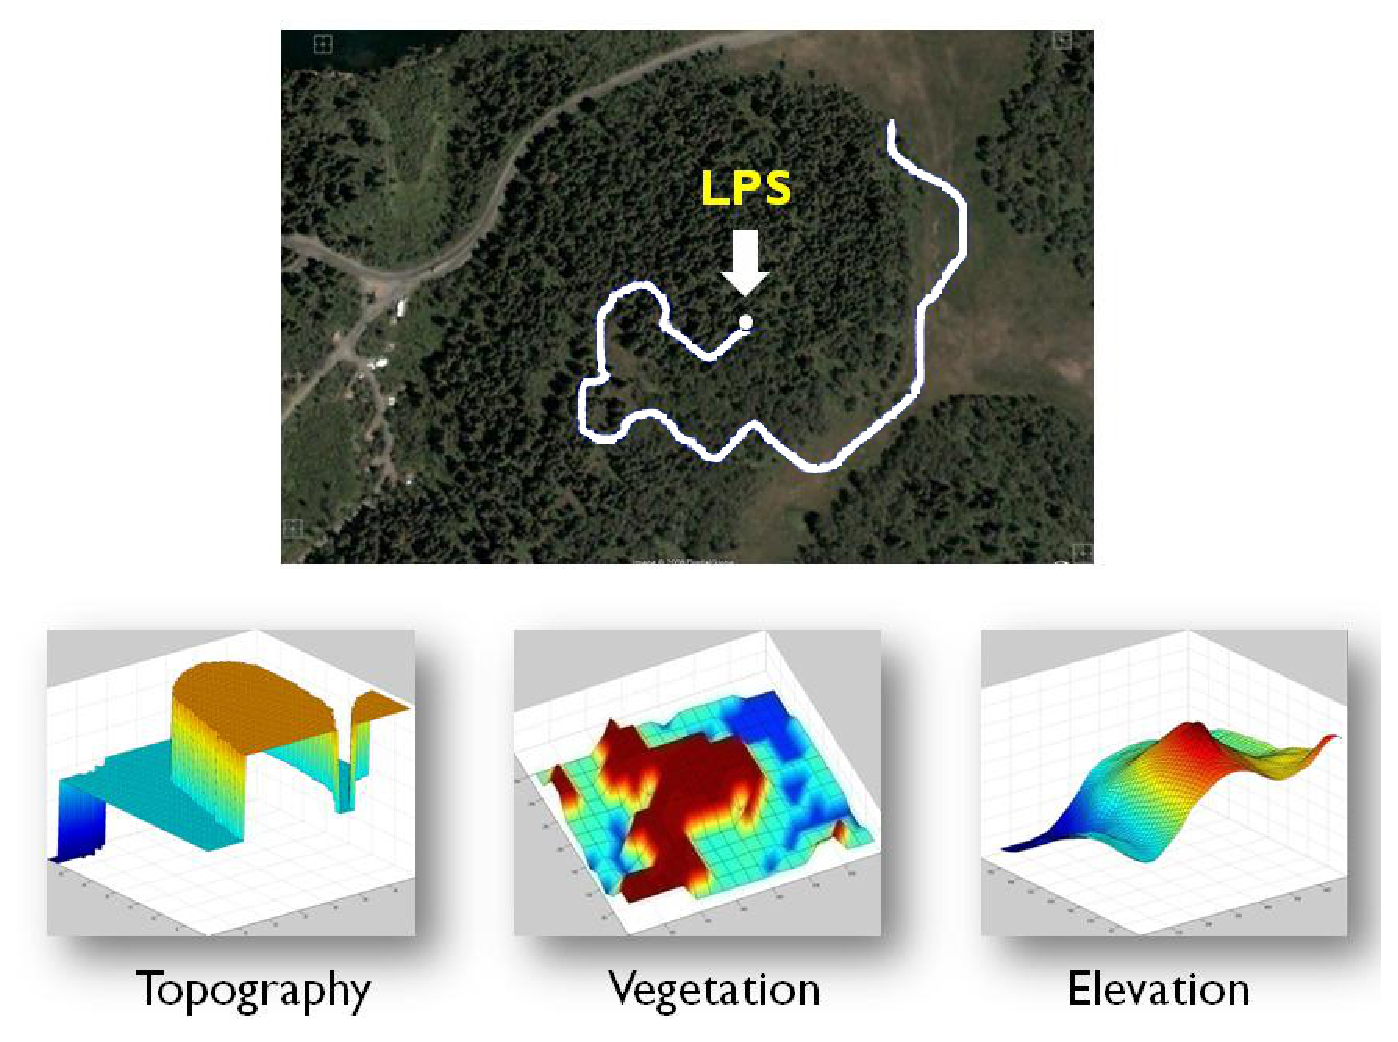
\includegraphics[width=4.5in]{satellite.eps}
\caption[Satellite imagery and terrain data of area by Payson Lake, Utah]{Satellite imagery of area by Payson Lake, Utah together with relative topography, vegetation, and elevation data downloaded from USGS web site. The topography and vegetation plots are discretized into (lake, plain, hill), and (sparse, medium, dense) respectively.}
\label{satellite}
\end{figure}

%---------------------------------------------------
\subsection{Hexagonal Tessellation Discretization}
\label{sec:3.3}

The first step in the model is to discretize the area into a hexagonal tessellation as shown in Figure~\ref{hexgrid}. The reason we use a hex tessellation is because the hex tessellation ensures the distance from the center of one cell to the center of any neighboring cell is always the same. The width of each hex cell is 24 meters. We picked this number because we believe such a granularity allows us to have enough detailed information about the terrain features without going into excessive details to burden the amount of computation. Future work should systematically explore how changing this granularity affects the tradeoffs between computational complexity and precision. In a real WiSAR scenario, the width can also be determined by the level of detail available for the terrain feature data at hand.

\begin{figure}
\centering
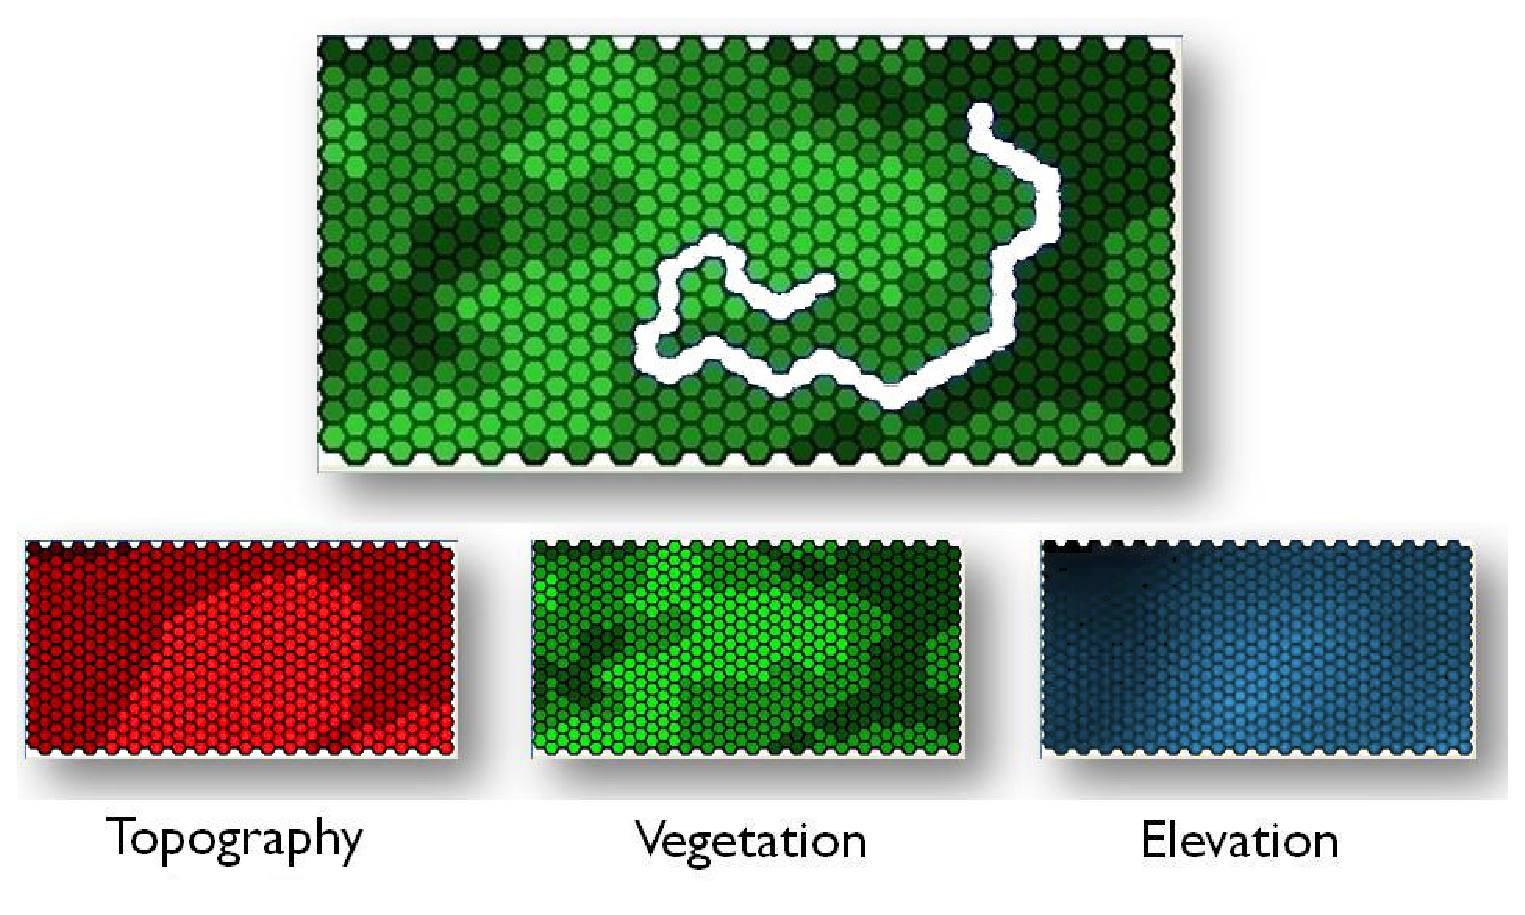
\includegraphics[width=4.5in]{hexgrid.eps}
\caption[Hexagonal discretized tessellation showing past historical data]{Hexagonal discretized tessellation showing past historical data (the path marked by the white cells in the main image) together with topography, vegetation, and elevation information in hexagonal tessellation.}
\label{hexgrid}
\end{figure}

The resulting tessellation is a $16 \times 38$ tessellation with 608 distinct states. Using the terrain feature data we have, each state is really a 3-tuple of (topography type, vegetation type, elevation). When we transition from one state to another neighboring state (including remaining in the same state), we can identify whether the topography type and vegetation type change. By calculating the elevation difference between the two states, we can find out whether the local slope is going uphill, downhill, or neither. Here we decide whether there is a local slope by calculating the angle of the elevation difference. If the difference is more than 20 degrees, we mark it as a local slope. We subjectively picked the threshold of 20 because we want to emphasize the extra effort of going uphill (as might be representative of a typical missing person such as a 14-year-old scout). Future work should systematically evaluate the impact of this threshold on usefulness of the probability distribution function.

%---------------------------------------------------
\subsection{Model Representation}
\label{sec:3.4}

In this sub-section, we define the Bayesian model in terms of the prior, the state transition, and the likelihood, and discuss each component in detail.

%*****************************
\subsubsection{The Prior}
\label{sec:3.4.1}

With the knowledge of past WiSAR incidents and expert opinion on human behavior, we can ask domain experts to specify their prior beliefs on how the missing person would behave with respect to different terrain features (e.g., a transition from a medium vegetation type to a dense vegetation type). For example, since we have three different topography types, we need a $3 \times 3$ transition matrix as shown in Equation~(\ref{matrix}), representing the probability of transitioning from one topography type to another. The rows and columns are both indexed by the different topography types, and it is possible to remain in the same topography, yielding
\begin{equation}
\left[
\begin{array}{ccc}
T_{00}' & T_{01}' & T_{02}'\\
T_{10}' & T_{11}' & T_{12}'\\
T_{20}' & T_{21}' & T_{22}'\\
\end{array}
\right]
\label{matrix}
\end{equation}
For example, $T_{00}'$ is the transitional probability for remaining in the lake type topography, and $T_{00}'$ is a number between 0 and 1 inclusive. The definition of the transition matrix requires that the values in each row of the matrix sum up to 1.

However, we would also like to enable the domain experts to incorporate uncertainty in their beliefs. Therefore, for each topography transition, instead of a number, a continuous Beta distribution is used, and a probability value, such as $T_{00}'$, can be generated by sampling from the Beta distribution. We use a Beta distribution because the domain of a Beta distribution's probability density function is $x \in [0; 1]$, which matches the parameter space of probability values. The curves of the Beta distribution also have the shape we desire because the mean and the mode of the curve can shift between 0 and 1 with various variances depending on what parameters we pick (illustrated in Figure~\ref{BetaPDF}). To specify uncertainty, for each topography transition probability, we ask the domain experts to provide a mean and a variance because these parameters are much easier to understand for non-statisticians compared to the $\alpha$ and $\beta$ parameters for the Beta distribution. Then we solve for the $\alpha$ and $\beta$ parameters automatically.

\begin{figure}
\centering
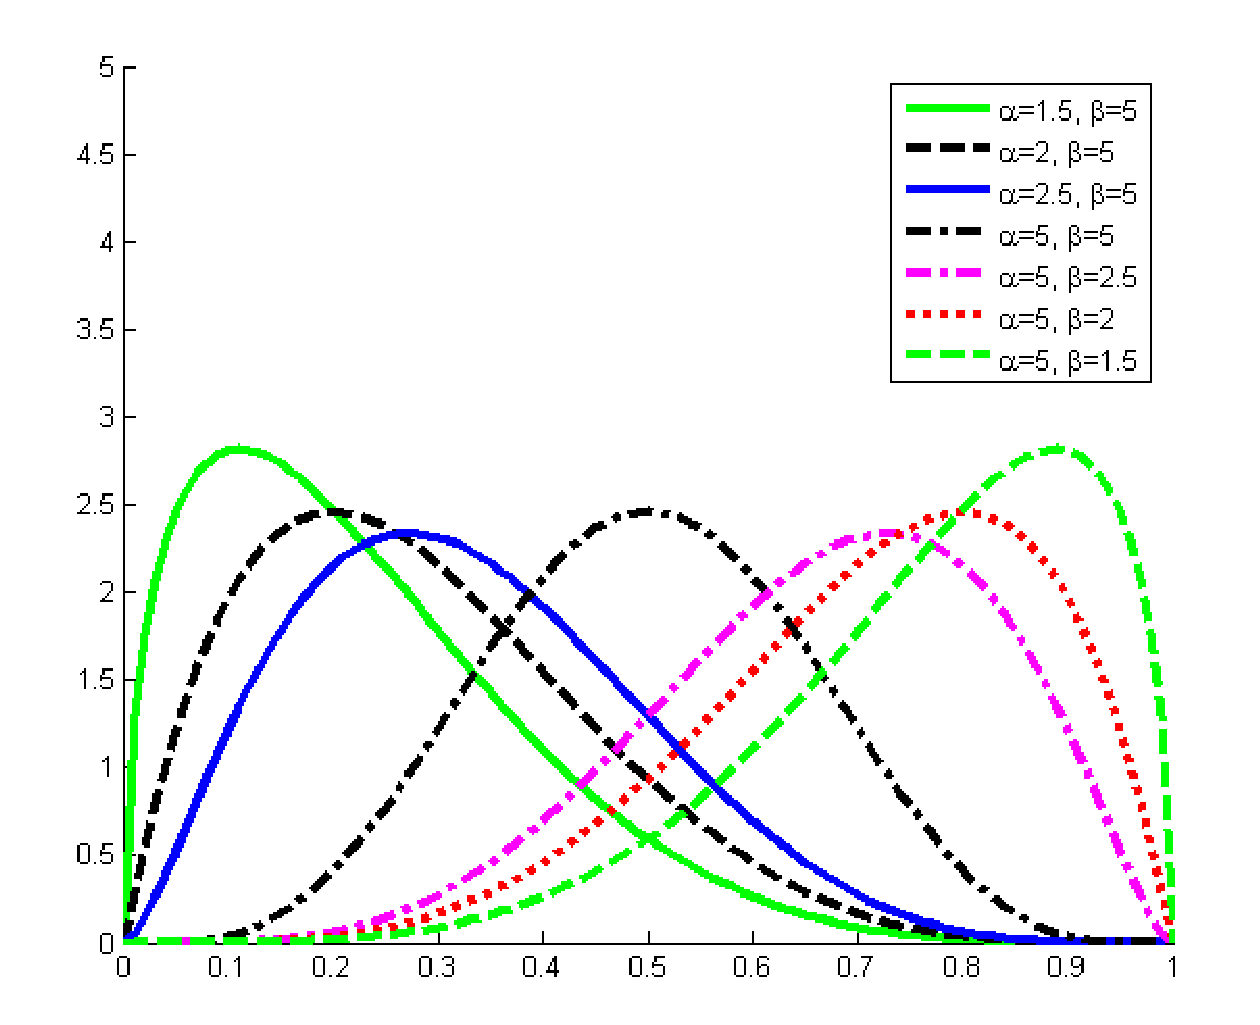
\includegraphics[width=3.5in]{BetaPDF.eps}
\caption[Beta Distribution probability density function]{Beta Distribution probability density function}
\label{BetaPDF}
\end{figure}

We have to be careful here to make sure the transition matrix, shown in Equation~(\ref{matrix}), is still valid. For example, the domain experts can specify means for Beta distributions relating to transitioning from topography type ``plain'' to all three topography types as 0.5, 0.3, and 0.2. These numbers sum up to 1. Unfortunately when we sample from the three Beta distributions, the values we get could possibly be something like 0.5, 0.35, and 0.22, which do not sum up to 1. That means these numbers are not true probability values, and we have to normalize them so they become true probability values. Therefore, we use $T_{ij}$ to denote the value we generate from the Beta distribution corresponding to transitioning from topography feature $i$ to topography feature $j$, and use $T_{ij}'$ to denote the true probability value (after normalization) for the transition. The probability distributions of $T_{ij}$ are the domain experts' prior beliefs with respect to topography terrain features, and there are 9 of them.

Similarly, since we have three different vegetation density types, we also need a $3 \times 3$ transition matrix to represent the probability of transitioning from one vegetation density type to another. This adds 9 vegetation density related priors to the model. With respect to local slopes, since there are only three possible transitions (uphill, no slope, and downhill), there are only 3 more priors to specify.

Therefore, our model has a total of 21 priors (9 related to topography, 9 related to vegetation density, and 3 related to local slope). For simplicity, we denote the joint distribution of all the priors as $\pi(\underline{\theta})$, where 
\begin{align}
\label{21}
\underline{\theta} &=T_{00},T_{01},...,T_{22},V_{00},V_{01},...,V_{22},S_0,S_1,S_2
\end{align}
and each prior follows a Beta distribution with known $\alpha$ and $\beta$ values (solved using the mean and variance values provided by domain experts). Thus
\begin{align}
\label{BetaT}
T_{ij} \sim Beta(\alpha_{T_{ij}}, \beta_{T_{ij}})\\
\label{BetaV}
V_{ij} \sim Beta(\alpha_{V_{ij}}, \beta_{V_{ij}})\\
\label{BetaS}
S_{i} \sim Beta(\alpha_{S_{i}}, \beta_{S_{i}})
\end{align}
where $T_{ij}$ represents the probability of transitioning from topography type $i$ to $j$ (possibly $i=j$) where $i=0,1,2$ and $j=0,1,2$. Similarly, $V_{ij}$ represents the probability of transitioning from vegetation type $i$ to $j$, and $S_{i}$ represents the probability of following a certain local slope type $i$.

%*****************************
\subsubsection{State Transition}
\label{sec:3.4.2}

In an earlier part of the paper we described how the search area is discretized into a hexagonal tessellation. Each cell becomes a state. Let $X$ represent a state, then $X$ can be defined as a vector containing information about the hexagonal cell:\\

\indent{}$X$ = [topography, vegetation density, elevation, index of tessellation]\\

With our model, we assume the state transition follows a first-order Markov process, meaning that the next state the lost-person (LP) will be in is only dependent on the current state the LP is in.
\begin{align}
\label{FirstOrder}
P(X_t|X_0, X_1, ..., X_{t-1}) = P(X_t|X_{t-1})
\end{align}

This is a strong assumption and it might not hold. For example, the amount of time traveled following the same direction (e.g., 20 minutes) could affect whether the LP wants to turn around and backtrack; similarly, the intended destination might affect which path the LP chooses while looking for the way. However, we argue that because the LP is in a disoriented state (although the LP might think otherwise) in the wilderness, the direction the LP follows could very well not be the direction the LP thinks he/she is following. Therefore, this assumption should not prevent the model from having useful predictive power. However, we also plan to extend the model in future work that will take into consideration the intended destination and incorporate that information into the representation of the current state.

When we compute $P(X_t|X_{t-1})$, it is necessary to combine the topography transition probability with vegetation density and local slope so we can borrow strength from each of the terrain features. We denote $T(Y|X)$ as the probability of transitioning from the topography of state $X$ to the topography of state $Y$, and $V(Y|X)$ as the probability of transitioning from the vegetation density type of state $X$ to the vegetation density type of state $Y$. Using the elevation difference between state $X$ and state $Y$, we can identify the local slope of going from state $X$ to state $Y$. We denote $S(Y|X)$ as the probability of transitioning from state $X$ to state $Y$ only based on local slope information. $T(X|Y)$, $V(X|Y)$, and $S(X|Y)$ are all true probability values, and they correspond to the relevant entries in the terrain features transition matrices such as Equation~(\ref{matrix}). Assuming the three terrain features are independent of each other we can combine the three probabilities by taking the product of the three,
\begin{align}
\label{product}
P(X_t|X_{t-1}) \propto T(X_t|X_{t-1})V(X_t|X_{t-1})S(X_t|X_{t-1}),
\end{align}
where $P(X_t|X_{t-1})$ is the entry in the row indexed by $X_t$ and the column indexed by $X_{t-1}$ in the state transition matrix describing the probability of transitioning from any state to any other state (including transitioning into the same state). Here $P(X_t|X_{t-1})$ is a true probability value.

Because a person can only travel from one hexagonal cell to its neighboring cells (or remain in the original cell), in each row of the state transition matrix, the transitional probabilities for all $X_t \notin N(X_{t-1})$ will be 0, where $N(X_{t-1})$ is the set of neighboring states of state $X_{t-1}$ (including $X_{t-1}$). That means the sum of $P(X_t|X_{t-1})$ for all $X_t \in N(X_{t-1})$ is 1 (elements in each row of the state transition matrix should sum to 1). 

If we look at each hex cell closely, we can see that from each cell a person can travel to one of the six neighboring cells or remain in the same cell. 
\begin{align}
\label{sub}
\mathrm{Let}~\underline{\phi'} &= P(X_t|X_{t-1}) ~\mathrm{where}~ X_t \in N(X_{t-1})\\
\mathrm{Let}~\underline{\phi} &= T(X_t|X_{t-1})V(X_t|X_{t-1})S(X_t|X_{t-1}) ~\mathrm{where}~ X_t \in N(X_{t-1})
\end{align}

We know $\underline{\phi}$ and $\underline{\phi'}$ each have 7 elements, and $\sum_{i=1}^7 \phi_i' = 1$, where
\begin{align}
\label{phi}
\phi_i' = \dfrac{\phi_i}{\sum_{j=1}^7 \phi_j}
\end{align}

Equation~(\ref{phi}) normalizes the products of terrain feature transition probabilities to compute the $P(X_t|X_{t-1})$ entries for all neighbors of state $X_{t-1}$.

%*****************************
\subsubsection{The Likelihood}
\label{sec:3.4.3}

Because from each cell a person can travel to one of the six neighboring cells or remain in the same cell, the likelihood of one observation (how the lost person traveled from one cell to one of the neighboring cells), denoted as $f(z|\underline{\theta})$, follows a categorical distribution with 7 dimensions. Relating to the previous section, $z$ can be defined as
\begin{align}
z = (X_t, X_{t-1}), ~\mathrm{where}~ X_t \in N(X_{t-1}).
\end{align}
In other words, $z$ is really a vector in the form of a 7-tuple, but to avoid notation confusion, we will only use $\underline{z}$ to denote multiple observations in a later section when we discuss posteriors. If we use $z_i$ to represent each element in vector $z$, then $z_i$ is constrained by
\begin{align}
\label{}
z_i \in \{0,1\} ~\mathrm{and}~ \sum_{i=1}^7 z_i=1,
\end{align}
meaning exactly one element in the 7-tuple is 1 and the others are all 0s. For example, an observation can be of the form of (0,0,0,0,1,0,0), meaning the person traveled to the fifth neighboring cell. Thus, our observation given all the prior beliefs is governed by
\begin{align}
\label{CAT}
z|\underline{\theta} &\sim CAT(\underline{\phi'}), ~\mathrm{where}\\
\underline{\phi'} &= \phi_1', \phi_2', ..., \phi_7', ~\mathrm{and}\\
%\end{align}
%\begin{align}
\label{likelihood}
f(z|\underline{\theta}) &= \prod_{i=1}^7 \phi_i'^{z_i},~\mathrm{where}\\
\underline{\theta} &= T_{00},T_{01},...,T_{22},V_{00},V_{01},...,V_{22},S_0,S_1,S_2.
\end{align}

Note that in order to compute the likelihood for $z$ using Equation~(\ref{likelihood}), we need to identify $X_{t-1}$, the state the person is in, and all neighboring states $X_t \in N(X_{t-1})$. We also need to sample from our priors $\pi(\underline{\theta})$ in order to construct terrain features transition matrices, which are then used in Equations~(\ref{sub}) --~(\ref{phi}) to compute $\underline{\phi'}$.

Figure~\ref{BN} illustrates the process of computing the likelihood graphically. The top row shows the 21 priors we sample from to generate $\underline{\theta}$ (9 for topography, 9 for vegetation density, and 3 for local slope). After normalization, we obtain all the entries for the terrain features transition matrices as shown in the second row (9 priors from the $3 \times 3$ topography transition matrix: $T_{00}', T_{01}', ..., T_{22}'$, 9 from the $3 \times 3$ vegetation density transition matrix: $V_{00}', V_{01}', ..., V_{22}'$, and 3 local slope probabilities: $S_0, S_1, S_2$). Depending on the $X_{t-1}$ and $X_{t}$ states associated with $z$, relevant $T(X_t|X_{t-1})$, $V(X_t|X_{t-1})$, and $S(X_t|X_{t-1})$ probability values are identified and multiplied to compute $\underline{\phi}$ (third row). The elements of the $\underline{\phi}$ vector are further normalized to produce $\underline{\phi'}$ (fourth row), which are the probabilities of the lost person traveling from state $X_{t-1}$ to all the neighboring states.

\begin{figure}
\centering
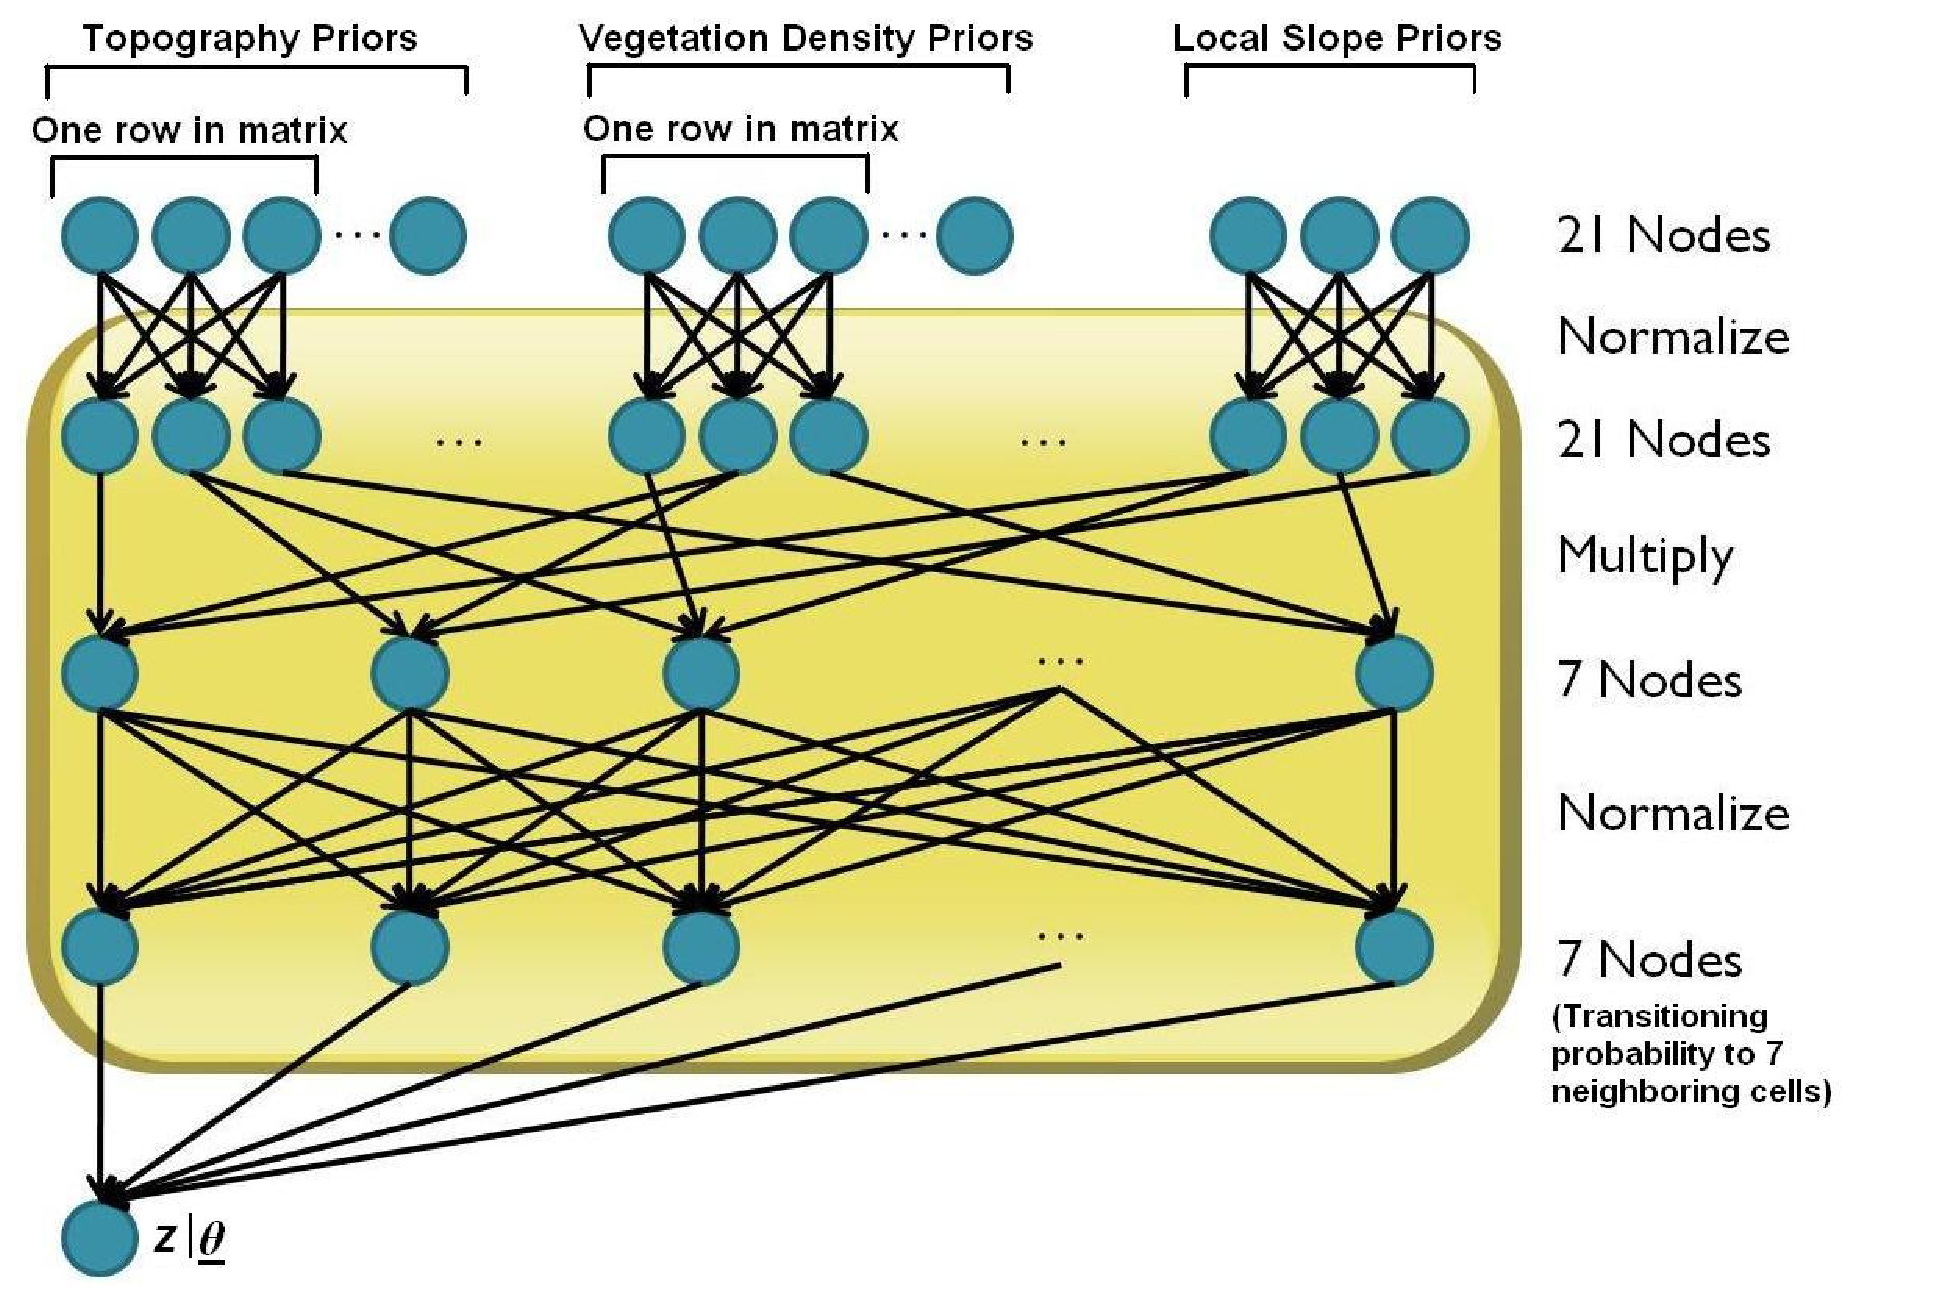
\includegraphics[width=4.5in]{BN.eps}
\caption{A graphical illustration of the proposed model. Top row: probability distribution for each prior belief. Fourth row: probability of transitioning into a neighboring cell in the hex tessellation. Bottom row: an observation indicating possible travel directions for the lost person.}
\label{BN}
\end{figure}

Once samples are generated from the priors $\pi(\underline{\theta})$, we can deterministically compute the values for the middle layers --- they are simply delta functions. Therefore, when we build the Bayesian network to compute the posteriors, we collapse all the middle layers and only keep the top and bottom layers.

%---------------------------------------------------
\subsection{Using the Model to Compute the Posterior}
\label{sec:3.5}

A great benefit of using a Bayesian model is that we can incorporate existing observations to update prior beliefs. The updated beliefs are the posterior beliefs.

Existing observations in the model are in the form of sections of GPS track logs (also discretized to a hexagonal tessellation) together with the terrain features associated with the track logs. By combining existing human behavior data with prior beliefs, we can reduce the domain experts' uncertainty.

To incorporate multiple observations, we simply add multiple $z|\underline{\theta}$ nodes in the bottom row of the Bayesian network (illustrated in Figure~\ref{BNPost}). The network is dynamically built with appropriate parent nodes identified and linked to the observation nodes dynamically.
\begin{figure}
\centering
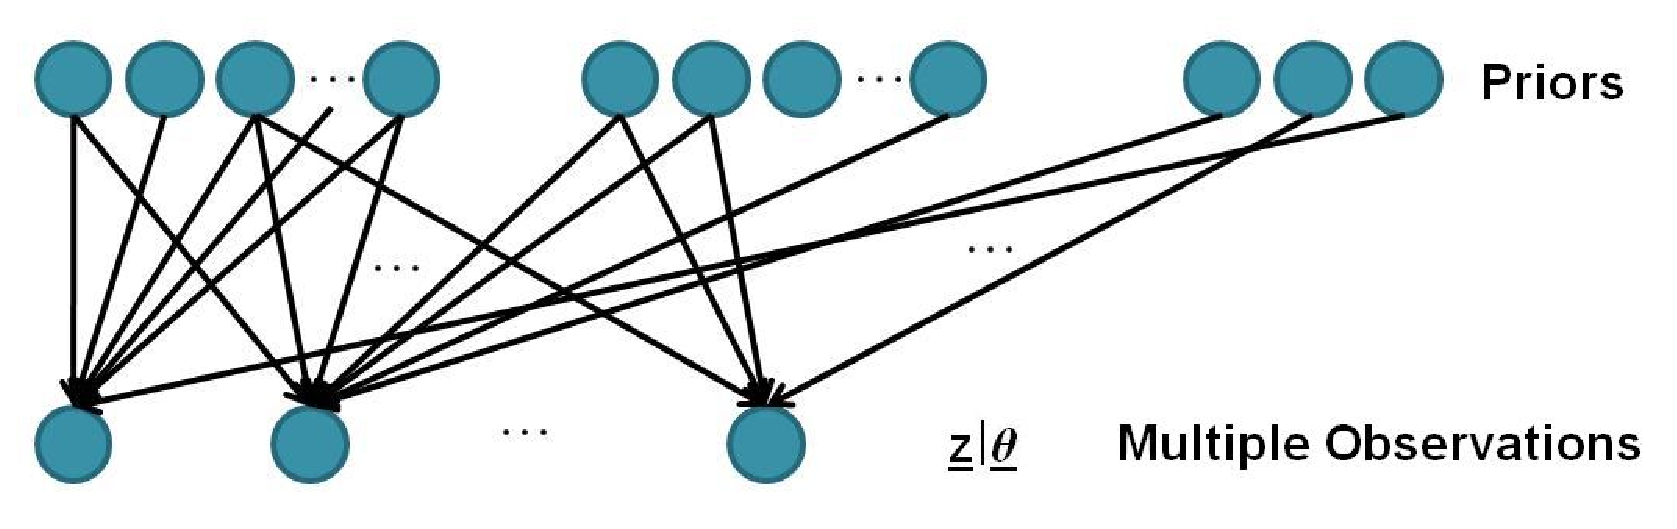
\includegraphics[width=4.5in]{BNPost.eps}
\caption{Bayesian network with multiple observations. Top row: probability distribution for each prior belief. Bottom row: multiple observations from previously collected human behavior data in the form of segments of GPS track logs together with terrain features associated with the track logs.}
\label{BNPost}
\end{figure}

Because of the complexity of the model, it is impossible to solve for the posterior distribution $\pi(\underline{\theta}|\underline{z})$ in closed form. That is why we used an MCMC approximation algorithm as the generation tool. Specifically, we used a random walk flavor of MCMC that uses the Gibbs Sampling algorithm, shown in~\cite{Gelman2004Bayesian}, on the outside loop, with Metropolis-Hastings algorithm, shown in~\cite{Gelman2004Bayesian}, inside each iteration of the Gibbs Sampling. Gibbs sampling is an algorithm for generating samples from a joint probability distribution of multiple random variables when the conditional distribution of each variable is known. It generates samples from the distribution of each variable in turn, conditioned on the current values of other variables. The Metropolis-Hastings algorithm generates a first-order Markov chain in each state and uses a proposal density, which depends on the current state, to generate a new proposed sample. This value is accepted if a value drawn from a uniform distribution between 0 and 1 meets certain requirements. Otherwise, the current value is retained. In our implementation, we used a Gaussian function as the proposal density.

In our implementation, we used 500 iterations for burn (throwaways) and kept 10,000 samples for each parent node. In each iteration, the Gibbs Sampling algorithm tries to sample from the distribution of each parent node in turn, conditioned on the current values of other parent nodes. However, Gibbs Sampling relies on the Metropolis-Hastings algorithm to really generate samples from the posterior distribution by using a proposal density function (a Gaussian distribution in our case). These samples approximate the posterior distribution for each of our 21 priors. 

Figure~\ref{Approximation} illustrates how the Monte Carlo method approximates the posterior distribution of one parameter (a parent node). In each iteration, the Metropolis-Hastings algorithm probabilistically generates a sample for the node based on the complete conditional constructed by Gibbs sampling (points inside smaller graphs in the upper portion where each point represents a probability value generated from a Beta distribution). If we combine all these samples into one graph and bin the points into small clusters (bigger graph in lower portion where the y axis is the count), we can connect the top of the bins and draw a curve. This curve is an approximation of the posterior distribution of the node, and as the number of samples approaches infinity, the curve matches the actual posterior distribution.

\begin{figure}
\centering
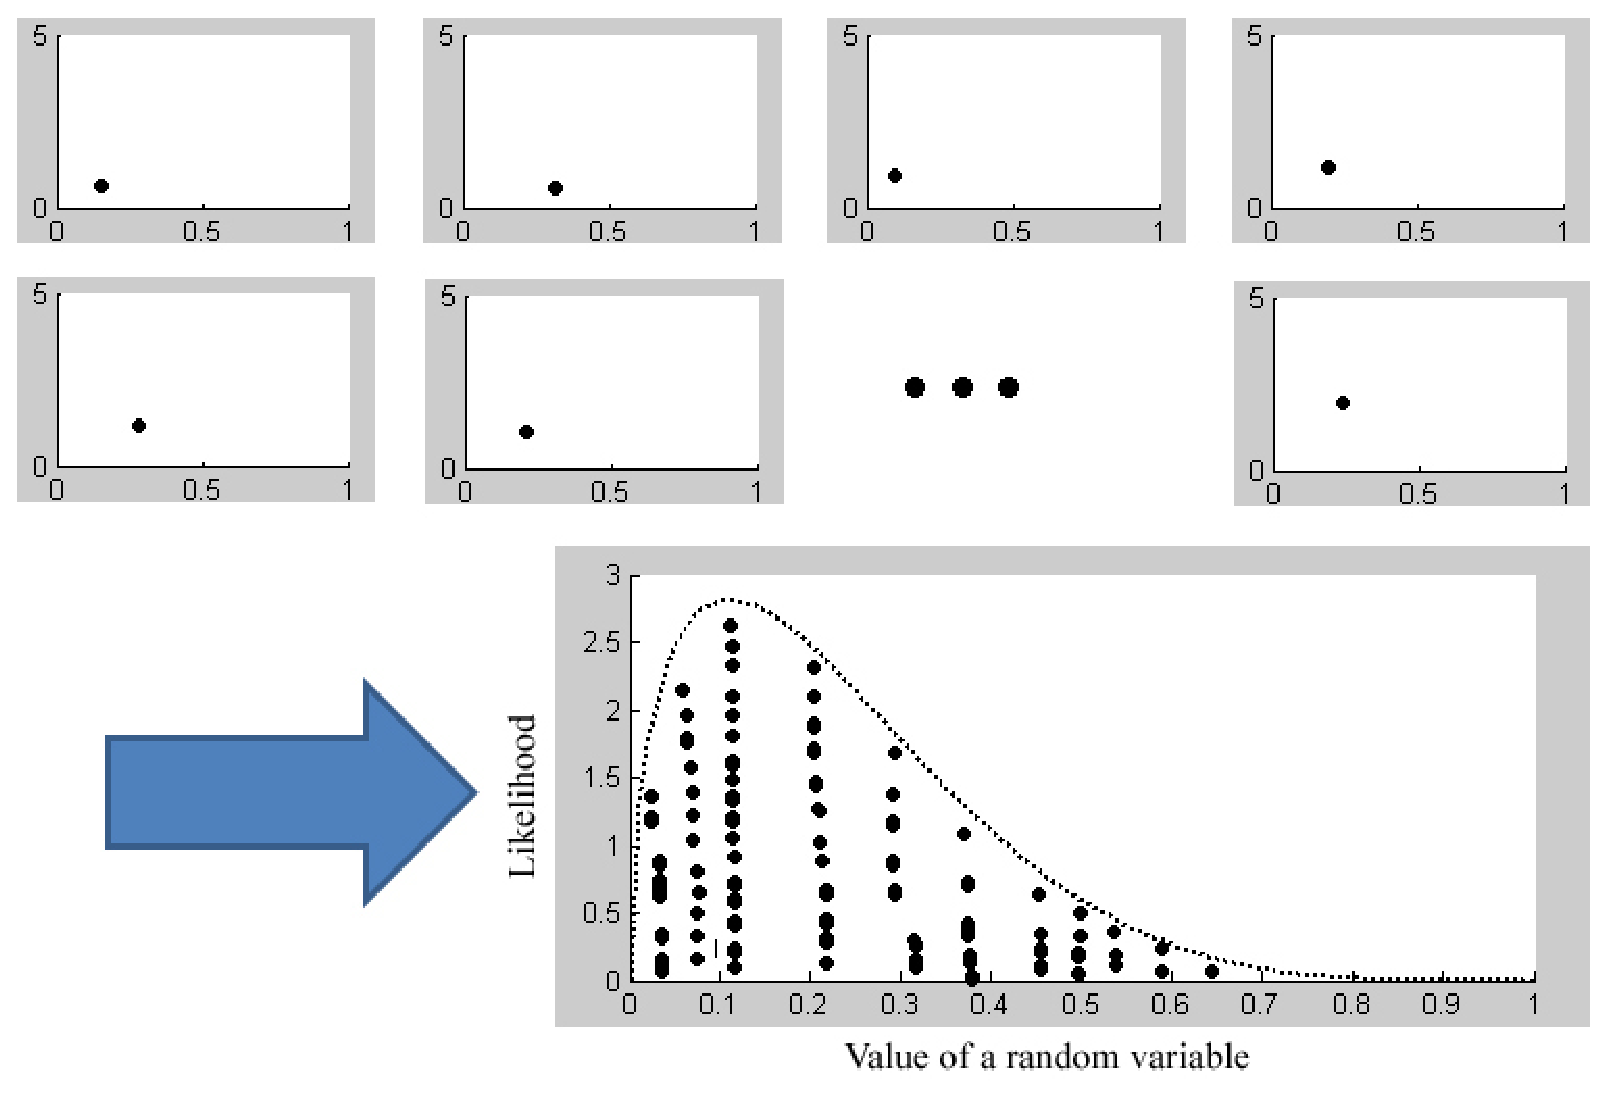
\includegraphics[width=4.5in]{Approximation.eps}
\caption{Graphical illustration of how the Monte Carlo method approximates the posterior distribution of one parameter. Upper: multiple iterations of sampling. Lower: samples clustered to approximate the real distribution.}
\label{Approximation}
\end{figure}

In our experiments, the MCMC algorithm completed in 220~seconds on a Dual-core AMD 3800+ PC with 3GB of memory.

%---------------------------------------------------
\subsection{Using the Model to Compute the Predictive Probability Distribution}
\label{sec:3.6}

Using the model described above, once we have the priors specified, we can build our $608 \times 608$ state transition matrix. In our implementation, we sample once from each Beta distribution for each time step. Starting from the lost person's point last seen, we can generate the prior predictive probability distribution by multiplying the state transition matrix in each time interval. This method allows the search and rescuers to see how the predictive probability distribution changes as time progresses.

~\cite{Setnicka1980Wilderness} and~\cite{Syrotuck2000Introduction} show that in WiSAR scenarios, as time progresses, the effective search radius increases by approximately 3km/hour, which is equivalent to 50m/minute. Because the age of the lost-person affects the speed the person travels, we can adjust the size of the time interval accordingly. With our lost scout scenario, because children generally travel slower than adults, we assume the lost scout travels at roughly 24m/minute; therefore, we define each time step as 1 minute. When we multiply the state transition matrix (sampled once from the prior distributions at each time step) 200 times (3 hours and 20 minutes = 200 minutes), we have the prior predictive probability distribution map as shown in the upper row of Figure~\ref{priorvspost}.

Once we combine previously collected human behavior data and approximate the joint posterior distribution of all the parameters, we can sample from the posterior beliefs instead of the prior beliefs. Following the same state transition matrix multiplication, we can also generate the posterior predictive probability distribution. The lower row of Figure~\ref{priorvspost} shows this distribution. In the Wilderness Search and Rescue case, the posterior predictive probability distribution is the 2D probability distribution map we are seeking.

\begin{figure}
\centering
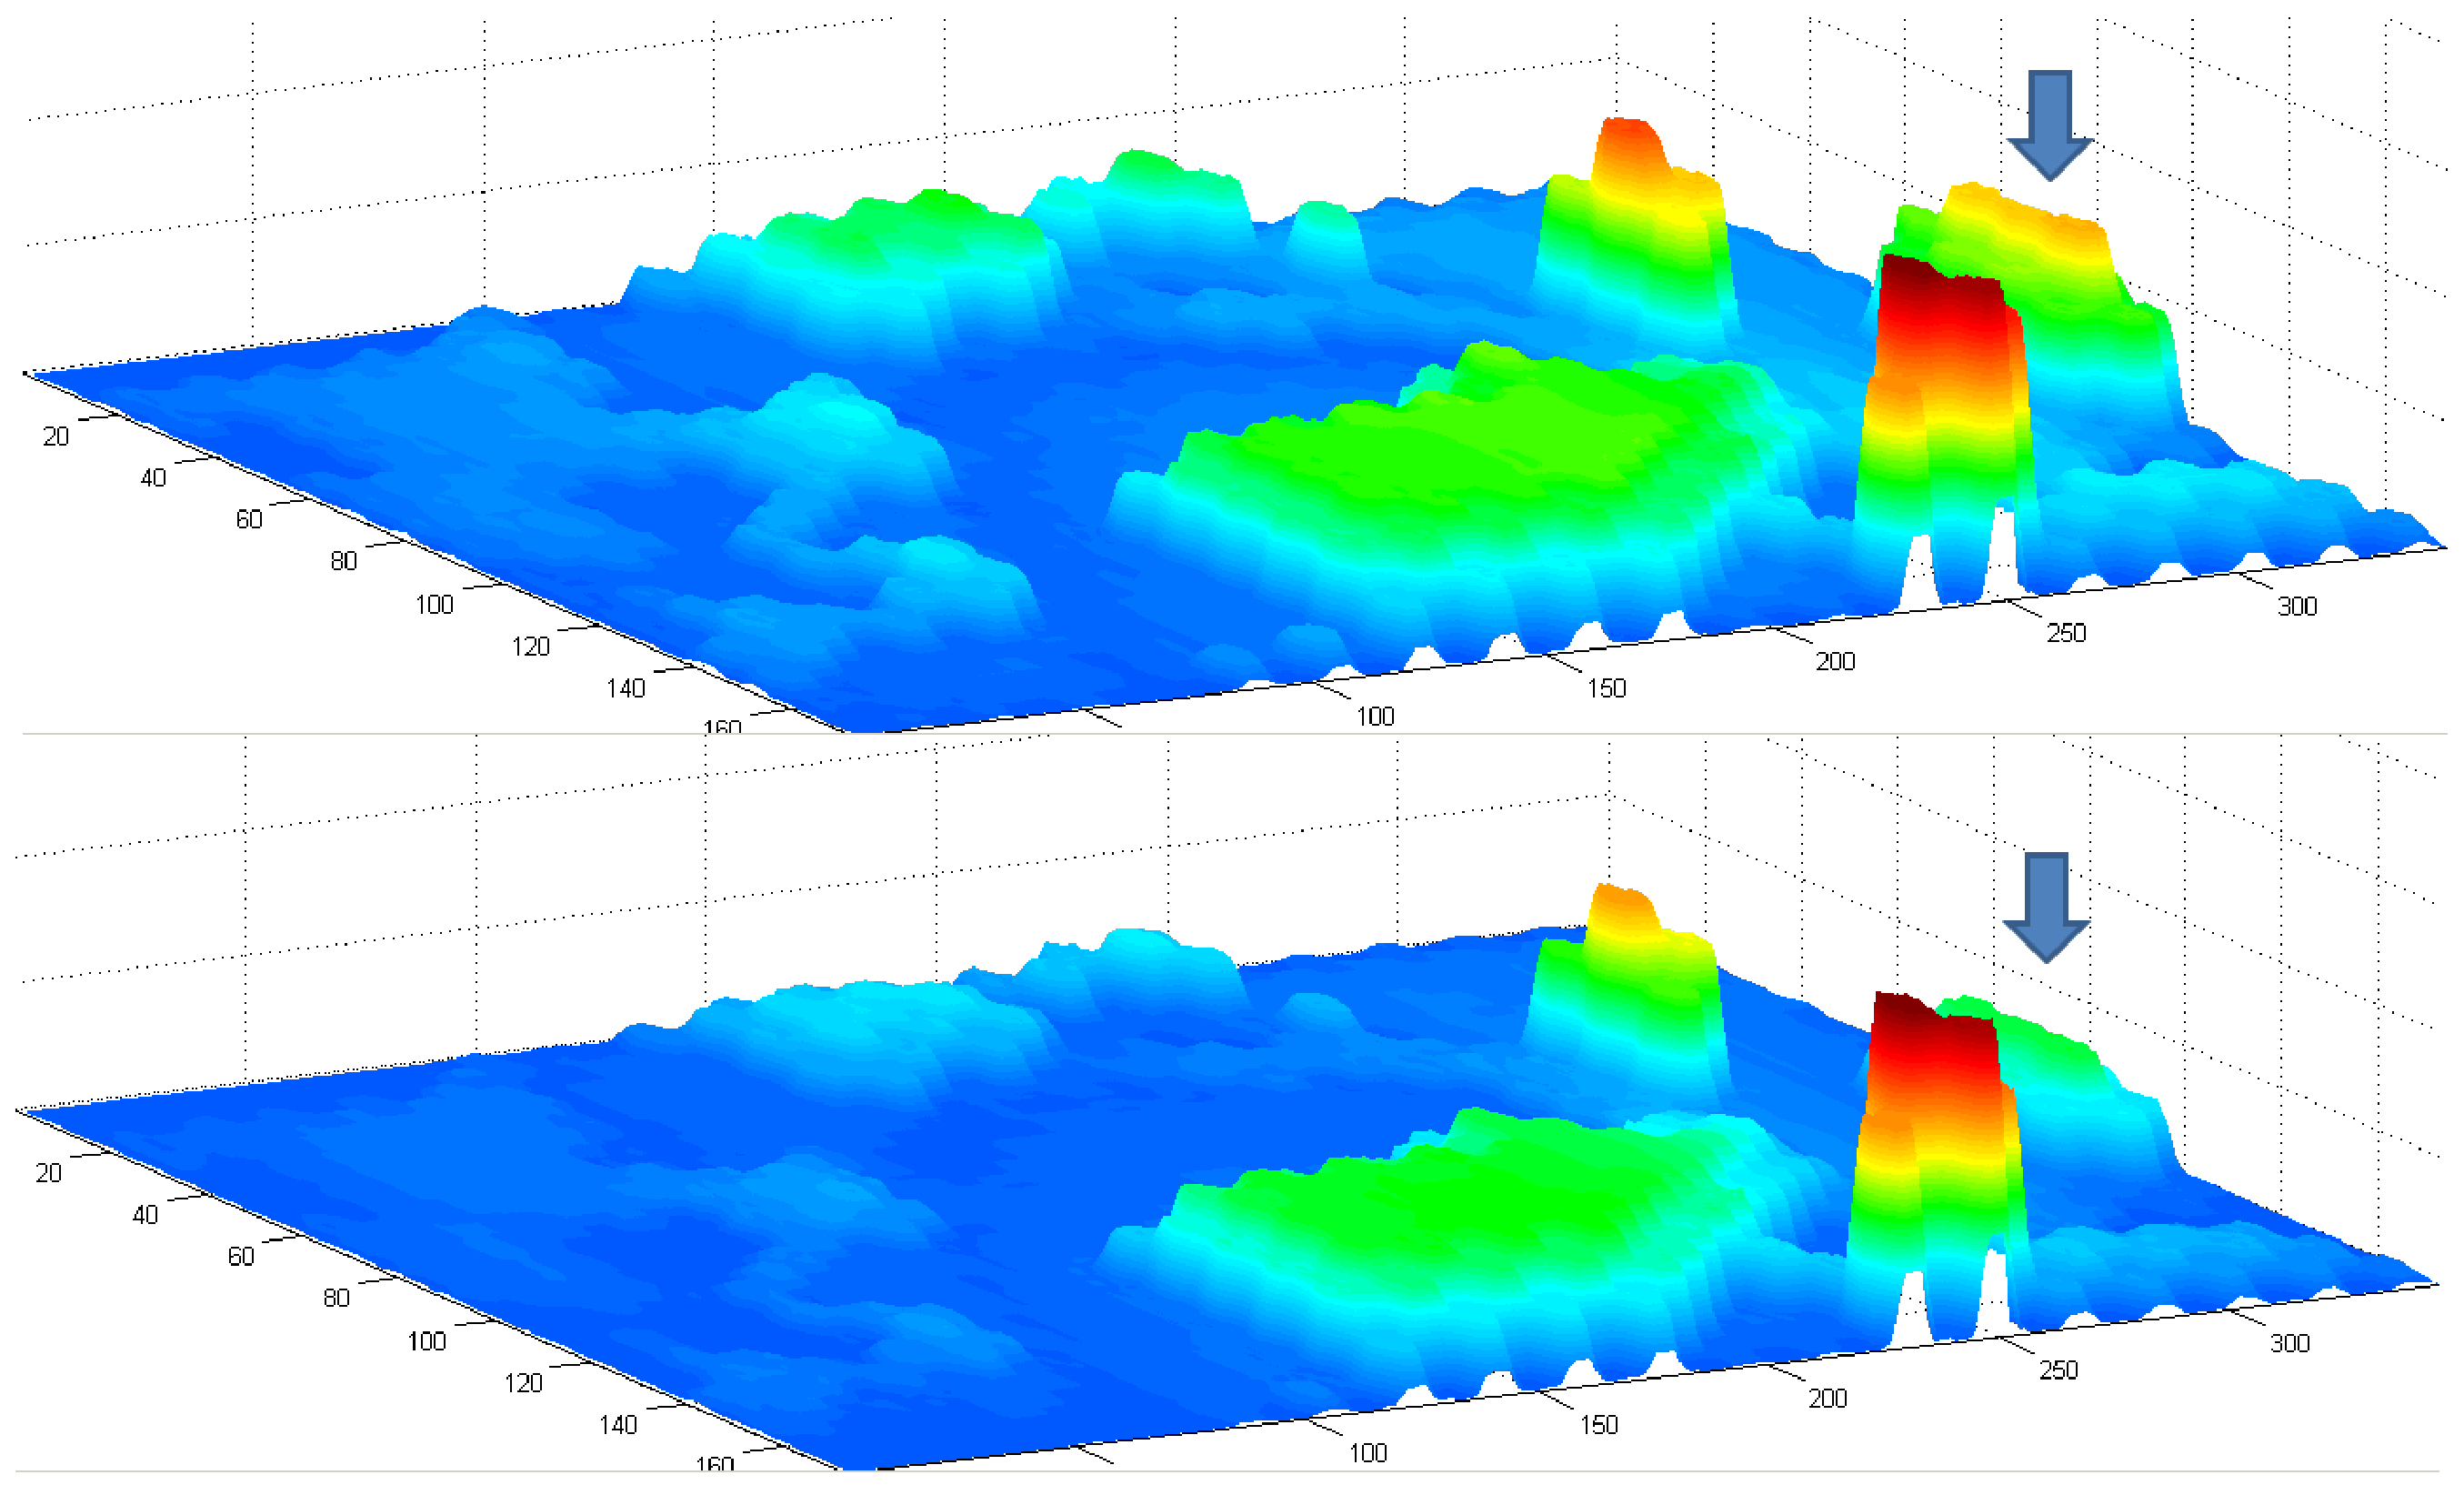
\includegraphics[width=4.5in]{priorvspost.eps}
\caption[Comparing prior predictive distribution against posterior predictive distribution]{Comparing prior predictive distribution (upper row) against posterior predictive distribution (lower row)}
\label{priorvspost}
\end{figure}

%=====================================================================================================
\section{Evaluation of the Model}
\label{sec:4}

%---------------------------------------------------
\subsection{Synthetic Data}
\label{sec:4.1}

Pretending to be domain experts, we specified all the prior distributions by setting the means and the variances. The matrices below show the prior distributions we set for the vegetation type transition matrix. The first matrix shows the means and the second matrix shows the variances.
\begin{equation}
\centering
\left[
\begin{array}{ccc}
\mu_{V_{00}}=0.6 & \mu_{V_{01}}=0.25 & \mu_{V_{02}}=0.15  \\
\mu_{V_{10}}=0.5 & \mu_{V_{11}}=0.3 & \mu_{V_{12}}=0.2  \\
\mu_{V_{20}}=0.4 & \mu_{V_{21}}=0.4 & \mu_{V_{22}}=0.2  \\
\end{array}
\right]
\end{equation}
\begin{equation}
\centering
\left[
\begin{array}{ccc}
\sigma^2_{V_{00}}=0.14^2 & \sigma^2_{V_{01}}=0.15^2 & \sigma^2_{V_{02}}=0.1^2 \\
\sigma^2_{V_{10}}=0.15^2 & \sigma^2_{V_{11}}=0.15^2 & \sigma^2_{V_{12}}=0.15^2 \\
\sigma^2_{V_{20}}=0.15^2 & \sigma^2_{V_{21}}=0.15^2 & \sigma^2_{V_{22}}=0.15^2 \\
\end{array}
\right]
\end{equation}

We set these values following common sense. For example, we believe a lost scout is more likely to remain in sparse vegetation type ($\mu_{V_{00}}=0.6$) and unlikely to transition from a sparse vegetation type to a dense vegetation type ($\mu_{V_{02}}=0.15$). We also believe a lost scout is more likely to transition from a dense vegetation type to a medium or sparse vegetation type and from a medium vegetation type to a sparse vegetation type ($\mu_{V_{21}}=0.4$, $\mu_{V_{20}}=0.4$, $\mu_{V_{10}}=0.5$). However, for most of these Beta distributions, we are not certain about our estimation, which is why we specified large variances for most of the parameters. For example, $\sigma^2_{V_{10}}=0.15^2$ means we believe the probability to transition from vegetation type medium to sparse could be as low as 0.05 and as high as 0.95. In real WiSAR scenarios, the priors should come from past statistical analysis of lost-person behaviors, such as~\cite{Heth1998Characteristics} and~\cite{Syrotuck2000Analysis}, combined with domain experts' opinions.

Each observed data point is a transition from one cell to another neighboring cell (including remaining in the same cell) in previously collected GPS track logs. The track logs do not even have to be in the same search area of the current incident. What we really care about is how terrain features affect a person's behavior in the wilderness. If the track logs contain this kind of information, we can use it to update our prior beliefs. These posterior beliefs can then be used in a generative approach to predict how the lost person might travel from the point last seen as time progresses. For the lost scout scenario, our observed data is partly shown in Figure~\ref{hexgrid} as the path of white cells. We use the word ``partly'' because during the travel, the person sometimes stayed in the same state during the 1-minute time interval. To test the robustness of the model, we intentionally designed the data set so that the person remained in the same vegetation type most of the time. We also repeated the same path three times in our synthetic dataset to simulate three different past GPS track logs. By repeating these we are basically adding more strength to the data and we expect the data to have a much stronger effect on the posterior distributions for the parameters. Each path consists of 45 transitions; therefore, our dataset has 135 data points.



%We are currently in the process of collecting real human behavior data in the form of GPS track logs from hikers\footnote{http://alltrails.com/}, hunters, and geocachers\footnote{http://tanglefoot.cs.byu.edu/~amy/index.html}. Note that historical datasets from different areas can be used together to generate posterior distributions for the same set of parameters, but samples generated from the posterior distributions will be used on the same search area in order to generate predictive distributions.

%---------------------------------------------------
\subsection{Prior vs. Marginal Posterior}
\label{sec:4.2}

Using the posterior samples, we can compare the marginal prior distribution with the marginal posterior distribution for each of our parameters. Figure~\ref{posts} shows the comparison for some of the parameters. The dotted lines represent the prior distributions and the solid lines represent the posterior distributions.

The plot in the upper left is for parameter $T_{02}$, the terrain feature transition probability from lake to hill. Since we do not have any data point in our dataset that transitioned from lake to hill, here we see the posterior is almost identical to the prior. The plot in the upper right is for parameter $T_{12}$, the terrain feature transition probability from plain to hill. In our dataset, a good segment of the path basically followed the contour line but stayed in the plain states. This characteristic of the dataset explains why the posterior distribution is much narrower and had a much lower mean---because the data did not show many changes from plain to hills, the posterior probability of this transition is much lower with less variance. The plot in the lower left is for parameter $V_{01}$, the terrain feature transition probability from vegetation type sparse to medium. The plot in the lower right is for parameter $S_1$, the terrain feature transition probability from no slope to no slope. Both of these posteriors are only slightly different from the priors.
\begin{figure}
\centering
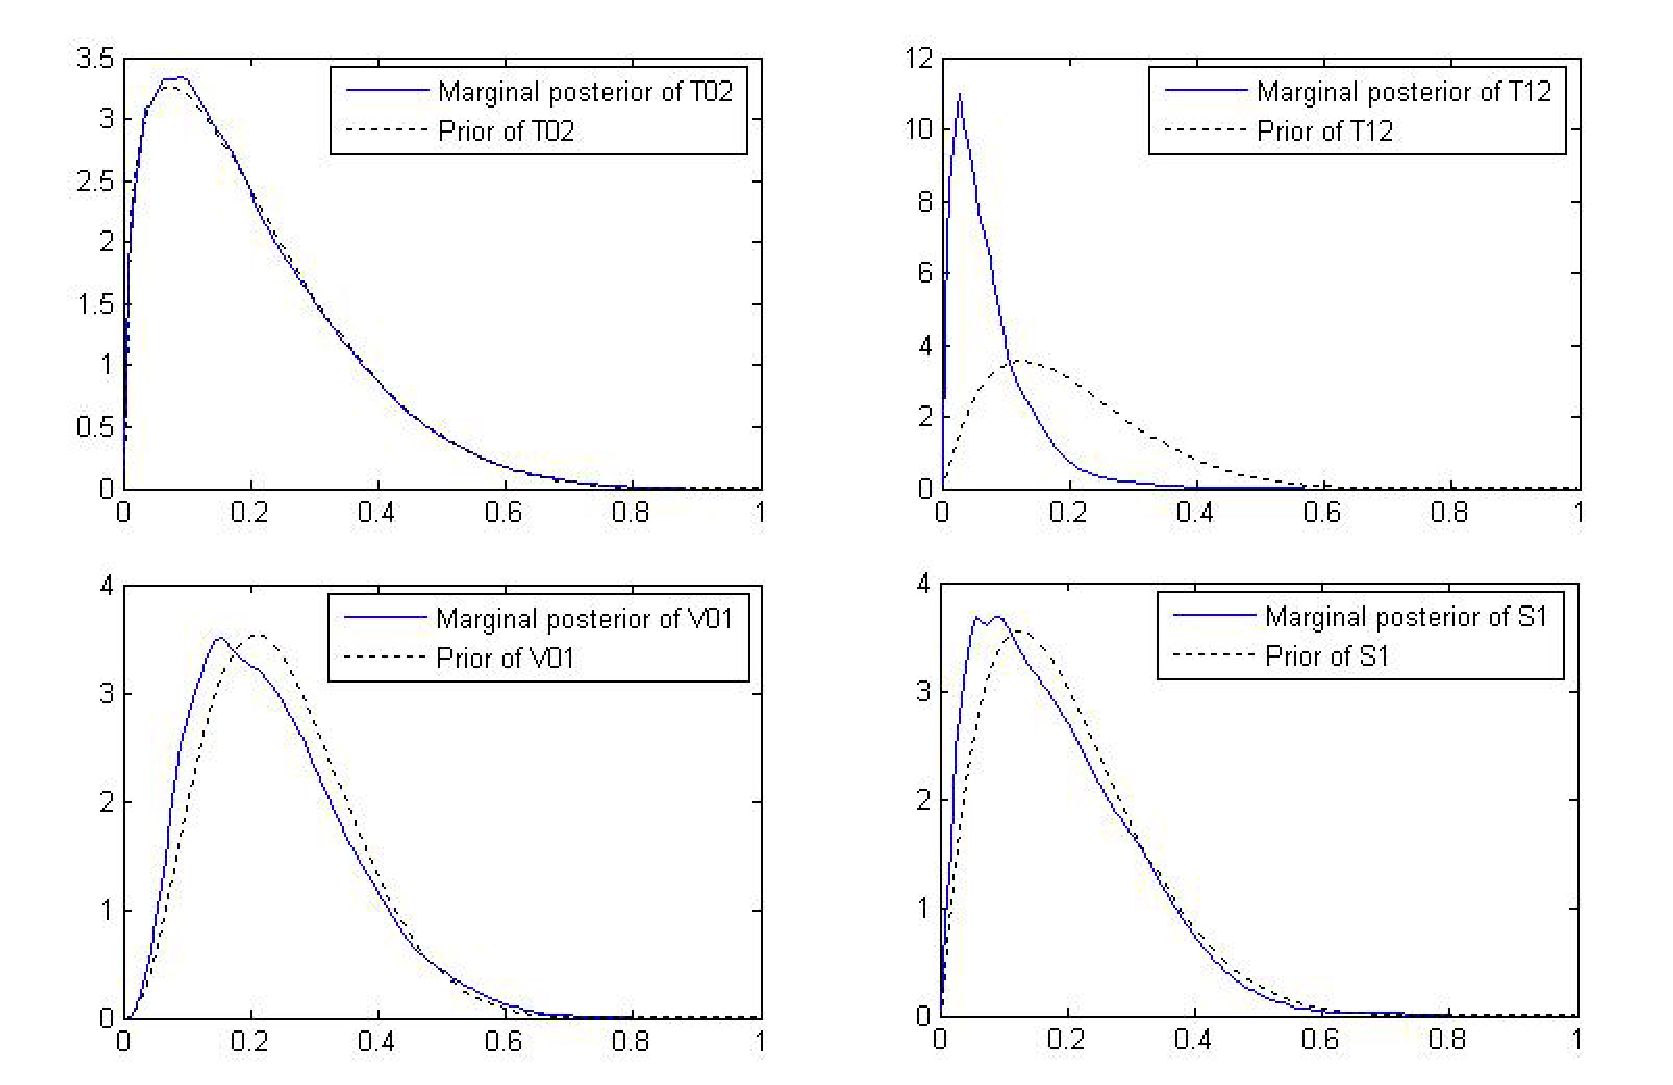
\includegraphics[width=5in]{posts.eps}
\caption[Comparing prior distribution with marginal posterior distribution]{Comparing prior distribution with marginal posterior distribution. Upper Left: $T_{02}$ Upper Right: $T_{12}$ Lower Left: $V_{01}$ Lower Right: $S_1$.}
\label{posts}
\end{figure}

%---------------------------------------------------
\subsection{Correlation of Parameters}
\label{sec:4.3}

When we ask the domain experts to specify the priors, we assume the parameters are independent. Because we have 21 parameters, the joint posterior distribution in the parameter space is really a distribution with 21 dimensions, which is impossible to plot. Instead, we use a correlation image to show whether there exist correlations between pairs of parameters.

Figure~\ref{correlation} shows a graphical representation of the correlation between each pair of parameters. A grey value, such as cell(1,21) in the lower left corner, indicates that there is no correlation between the two parameters. A white cell, such as cell(1,1) in the upper left corner, means the two parameters are fully positively correlated, and a black cell means the two parameters are fully negatively correlated. Here we see that the vegetation parameters $V_{20}$ (dense to sparse), $V_{21}$ (dense to medium), and $V_{22}$ (dense to dense) showed positive correlation. Other positive correlations also mostly appear between neighboring parameters. There is also a clear positive correlation between $V_{22}$ (Vegetation: dense to dense) and $S_{0}$ (uphill). These positive correlations are marked by the big circle in Figure~\ref{correlation}.

The results of the correlation analysis indicate that there is likely a correlation among different terrain features. Interestingly, from this figure we can see that parameter $V_{12}$ (Vegetation: medium to dense) and $T_{11}$ (Topography: plain to plain) are clearly, negatively correlated (marked by the upper small circle in Figure~\ref{correlation}). Parameter $V_{22}$ (Vegetation: dense to dense) and $T_{11}$ (Topography: plain to plain) are also clearly, negatively correlated (marked by the lower small circle in Figure~\ref{correlation}). A closer look at the terrain features of the area shows that dense vegetation is mostly located on the hill topography type and medium vegetation is mostly located on the plain topography type. This explains why we see such a negative correlation. This emergence of correlations that are compatible with terrain features suggests that the process of combining prior information with observed track logs is useful. However, when we let the domain experts specify the prior distributions, it is much more intuitive for them to assume independence instead of specifying conditional probabilities (to specify how the parameters are correlated), and we rely on data to identify the dependence relationship.
\begin{figure}
\centering
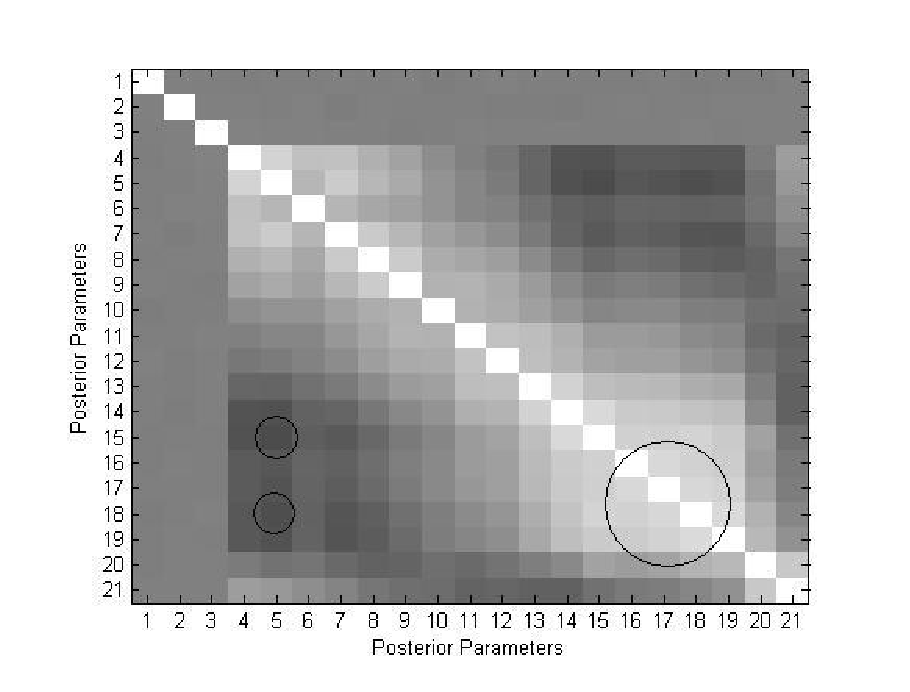
\includegraphics[width=4.5in]{correlation.eps}
\caption[Parameter correlation]{Parameter correlation: a grey value of 128, such as (1,21) in the lower left corner, represents no correlation. A white cell, such as (1,1) in the upper left corner, represents a correlation of 1. A black cell represents a correlation of -1. Parameters are in the following order: $T_{00},T_{01},...,T_{22},V_{00},V_{01},...V_{22},S_{0},S_{1},S_{2}.$} The big circle marks a positive correlation between parameters, and the small circles mark a negative correlation between parameters.
\label{correlation}
\end{figure}

%---------------------------------------------------
\subsection{Prior Predictive vs. Posterior Predictive}
\label{sec:4.4}

In this section we compare the prior predictive probability distribution and the posterior predictive probability distribution. The prior predictive is generated by sampling from the prior beliefs specified in the first part of the model. The posterior predictive is generated by sampling (using MCMC) from the posterior beliefs generated from the first part of the model. If no previous human behavior data is available, then the prior predictive can still be used to show likely places to find the missing person; otherwise, the posterior predictive should be used because combining existing human behavior data enables the model to reduce uncertainty in the posterior beliefs.

Both probability distributions use a generative approach to predict how the lost person might travel from the point last seen as time progresses. The 2D probability distribution map generated is the final product of the model and can be used by Incident Commanders in WiSAR operations.

The lower row of Figure~\ref{priorvspost} shows the posterior predictive distribution created using the samples generated for all the parameters through MCMC. After 200 time steps (equivalent to 3 hours and 20 minutes), we can see that near the right side of the map, clearly much less probability mass is allocated compared with the prior predictive distribution (indicated by arrows). The center of the northern region also has lower probability compared with the prior predictive distribution, but the difference is not dramatic. Therefore, with our lost scout scenario, this posterior predictive probability distribution map suggests that we should send search and rescue workers to the regions marked by the two highest peaks first to maximize the likelihood of finding the missing scout.

%=====================================================================================================
\subsection{Bayesian \texorpdfstring{$\chi^2$}{Chi-squared} Test for Goodness-of-Fit}
\label{sec:4.5}

We used the Bayesian $\chi^2$ test for goodness-of-fit proposed by~\cite{Johnson2004Bayesian} to evaluate the  quality of posterior beliefs in the proposed model. This test is closely related to the classical $\chi^2$ goodness-of-fit statistic, but different in many aspects. The classical $\chi^2$ goodness-of-fit test computes a single $p$-value. The Bayesian version, however, computes the goodness-of-fit at each iteration of the MCMC, conditional on the current set of model parameter values sampled from the posterior distribution of all the model parameters. The posterior distribution of the resulting $p$-values converges to a $\chi^2$ distribution with $k-1$ degrees of freedom as the number of iterations approaches infinity. \cite{Johnson2004Bayesian} defined the Bayesian $\chi^2$ test for goodness-of-fit using the following equation:
\begin{align}
R^B(\vec{\tilde{\theta}}) = \sum_{k=1}^K {\left [\dfrac{(m_k(\vec{\tilde{\theta}})-n p_k)}{\sqrt{n p_k}}\right ]}^2
\end{align}
where $\vec{\tilde{\theta}}$ is a set of model parameters sampled from the posterior distribution in a single iteration, $m_k(\vec{\tilde{\theta}})$ represents the number of observations that fell into the $k$th bin, $n$ is the total number of observations, and $p_k$ is the probability assigned by the null model to this interval. Values of $p_k$ are held fixed while the bin counts $m_k(\vec{\tilde{\theta}})$ are considered as random quantities.

Because our likelihood function is a categorical distribution with 7 parameters (a discrete distribution) we used 7 bins, so $k=7$. It is worth mentioning that $p_k$ is different for each data point in our case. For each set of model parameters, we calculate the probability values (for each neighbor of the cell, into which the data point fell) for the 7 bins for each observed data point, and then sum up all the probability values for each bin across all data points. By dividing the sum for all bins, we normalize the probability value, and the result is the probability for that bin.

With $k-1=6$ degrees of freedom, we computed the $\chi^2$ distribution and then computed the quantiles (the $p$-values) for each of the 10,000 $R^B(\vec{\tilde{\theta}})$ values. The results show that only 6 out of 10,000 $p$-values are smaller than 0.05, the statistical significance value we selected. The Bayesian $\chi^2$ test of goodness-of-fit suggests that our model fits the synthetic dataset well.

%=====================================================================================================
\section{Discussions and Limitations}
\label{sec:5}

First we summarize some of the assumptions made throughout the development of the model and our rationale behind them. We assume that the state transition follows a first-order Markov process. Our argument is that the lost person is likely in a disoriented state, therefore, the assumption should not be a big problem (see section~\ref{sec:3.4.2} for more details). Another assumption is that the three terrain features are independent. Although correlation analysis shows possible dependence between terrain features, we believe it is more intuitive for domain experts to assume independence instead of specifying conditional probabilities, and we rely on data to identify the dependence relationship (see section~\ref{sec:4.3} for more details). We also assume that the Markov process is stationary with homogeneous time steps (see section~\ref{sec:3.6} and section~\ref{sec:4.4}). However, we argue that the flexibility of specifying finer time intervals and the possibility to stay in the same state can ``simulate'' a non-stationary process with various time durations, thus alleviating the restriction.

After analyzing 162 lost-person incidents near Peter Lougheed Provincial Park in Alberta, Canada, \cite{Heth1998Characteristics} come to the conclusion that there is a close correlation between a lost-person's intended destination and the angle of dispersion (calculated from the lost-person's point last seen and the point the person was eventually found). This finding suggests that it might be a good idea to incorporate the missing person's intended destination into our existing model.

One limitation of this paper is that we are using synthetic data for our evaluation. To address this, we recently collected all the GPS track logs within the US that were uploaded to the popular web GPS track log repository, everytrail.com. We were able to identify 329 GPS track logs that contained the word ``geocache'' (or ``geocaching''). Because most of the geocache ``treasures'' are hidden in the wilderness off of a designated trail, we believe that GPS track logs created by geocachers are likely to contain behavior data indicating how a human might react to different terrain features. After closer examination of these track logs, we see a clear trend that the locations of the geocache ``treasures'' play an important role in the person's behavior in the wilderness in addition to terrain features. If we want to use this kind of GPS track log data as existing human behavior data, our model has to take into consideration the intended destination.

Another trend we observed from these GPS track logs is that a majority of the geocachers first followed some trails to get closer to the ``hidden treasure''. When the trail starts to clearly lead the person further away from the geocache, or when the person decides to take a shortcut somewhere along the trail, the geocacher then abandons the trail and creates a new path.

During the summer of 2009, a student in our research lab went for a geocache hunt near Box Elder Peak in Utah. After successfully finding the ``hidden treasure'', he decided to not return the same way he came from, but to try some alternative route. Soon he found himself lost and struggled for several hours to reorient himself. Eventually he stumbled onto a hiking trail, a different one from what he took before completing the geocache mission, then he followed the trail and found his way back. Figure~\ref{BoxElderPeak} shows the GPS track log displayed in Google Earth for the period when he was off-trail and lost in the wilderness. The point we want to make here is that after running into another unknown hiking trail, he immediately decided to stay on the trail. This kind of behavior can only be predicted by models that handle trail-following, and our present model clearly lacks this capability.

We plan to extend our model to support intended destination and trail-following. Doing so would allow us to take advantage of abundant GPS track logs and incorporate such human behavior data into the posterior distribution. Once we have the newer model, we can also take advantage of the existing Bayes factor analysis methods, such as Akaike Information Criterion (AIC) proposed by~\cite{Akaike1974AIC}, Bayesian Information Criterion (BIC) presented in~\cite{Schwarz1978BIC}, and Deviance Information Criterion (DIC) described in~\cite{Spiegelhalter2002DIC}, to perform extended validation.

In the present model, for every time step, only one sample is generated from each Beta distribution. A possible improvement is to use the idea of particles. At each time step, the model would generate, for instance, 100 examples from each Beta distribution, and then compute 100 sets of categorical distributions (each has 7 discrete values representing probabilities of transitioning to 7 directions), which can then be averaged to produce a final categorical distribution with better quality and a better representation of the experts' uncertainty. Because the added computation is outside of the MCMC algorithm and the matrix multiplications, the added execution time should be minimal.

Another important question we should ask is: How well would an experienced IC trust the probability distribution map generated using the proposed model? We strongly believe that the predictive probability distribution generated using the proposed model should only be used as a base onto which domain expertise can be further projected. The objective of the model is to provide a tool that reduces the IC's workload and supports the IC's operation, but not to replace the IC's responsibilities. With abundant experience, training, and the ability to incorporate much richer information (e.g., lost person profile, weather), the IC is responsible for validating the probability distribution suggested by the model and also for coming up with the final distribution map. To really make the tool useful for ICs in WiSAR operations, two additional elements are necessary: 1) a human factors analysis (user study) of the users' trust of the algorithms and automation in the WiSAR domain, and 2) an interface component/tool that enables the IC to easily modify the probability distribution generated by the model. The ability for the IC to modify the probability distribution both at the beginning and during the search can potentially improve how (much) users trust the system and make the proposed model more acceptable to users. Future work should develop an interface tool that enables a user to modify a probability distribution map. We believe results from such research can help improve the usability and usefulness of the proposed model.

\begin{figure}
\centering
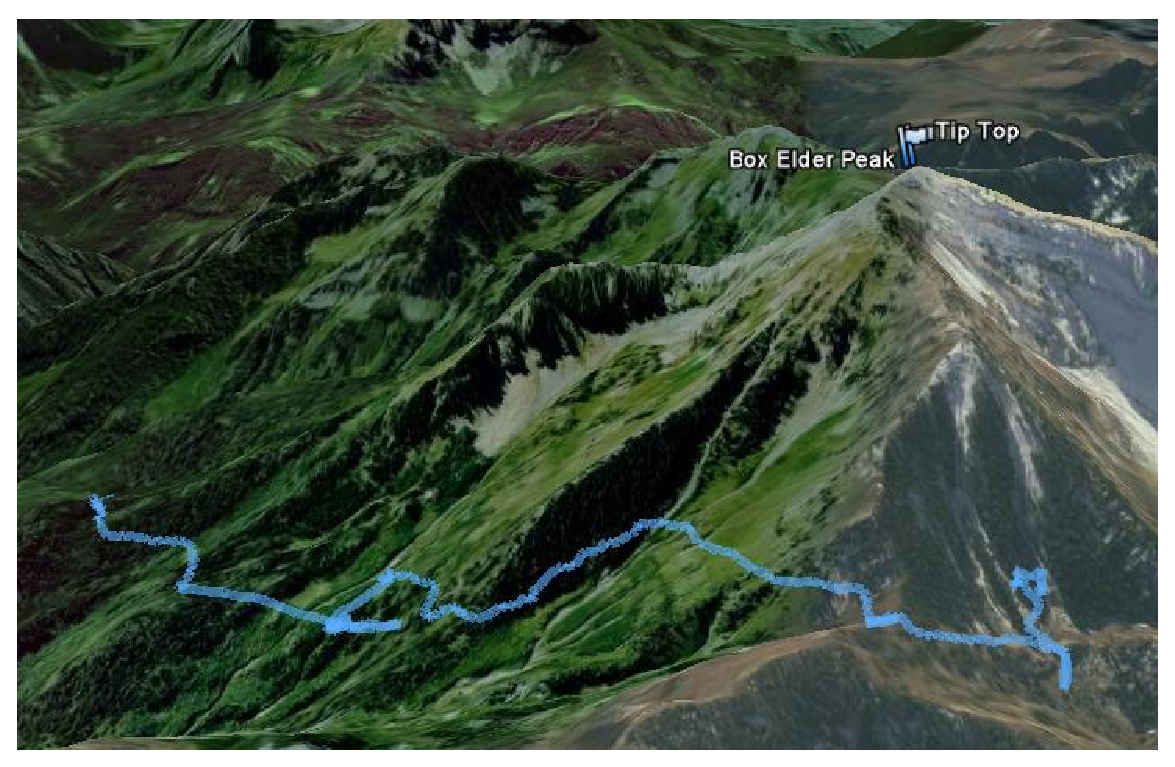
\includegraphics[width=3.5in]{BoxElderPeak.eps}
\caption[Satellite imagery of Elder Box Peak in Utah]{Satellite imagery of Elder Box Peak in Utah. The GPS track log shows the path taken by a hiker in summer 2009 when he went off the hiking trail and became lost for several hours before stumbling into another hiking trail.}
\label{BoxElderPeak}
\end{figure}



%=====================================================================================================
\section{Conclusions and Future Work}
\label{sec:6}

In WiSAR operations, the Incident Commander typically has limited resources and relies on a probability distribution map to allocate resources, to direct the search, and to coordinate rescue workers. Because as time progresses, the survivability of the missing person decreases and the effective search radius increases by approximately 3km/hour, it is critical to find the missing person quickly. That is why areas with high probabilities are searched first, and the quality of the probability distribution map can have a great impact on the search and rescue operations. We proposed a Bayesian approach to help generate such a probability distribution map by modeling lost-person behaviors based on three terrain features: topography, vegetation, and local slope. Our objectives are to ease the generation of probability distribution maps for the search and rescuers and to improve the quality of these maps.

Our proposed model uses publicly available geographic information and enables domain experts to specify uncertainty in their prior beliefs of how the missing person will transition from one terrain feature to another. Using the Bayesian model, past human behavior data in wilderness can be incorporated into the model to generate posterior beliefs. Following a first-order Markov process, the posterior beliefs can be used to build a temporal state transition matrix that allows the generation of the posterior predictive probability distribution map for any given time interval. We evaluated our model using the Bayesian $\chi^2$ test of goodness-of-fit from~\cite{Johnson2004Bayesian} because it allows the evaluation of multiple $p$-values for samples generated from the posterior parameter space. Results from the test suggest that our model fits the synthetic dataset well. The proposed Bayesian approach is promising, but we also acknowledge that the present model is limited to the proposed terrain features and could benefit from incorporating additional factors such as intended destination and trail-following.

In future experiments, we plan to let search and rescue experts specify terrain-based transitional probabilities so the prior predictive probability distribution can be generated using our model. Then we also let the experts directly specify a probability distribution on the regional map (with and without the restriction of only considering how terrain features would affect the lost-person's behavior). It would be very interesting to compare the resulting distributions and analyze the causes of any differences. However, because there is no ``ground truth'' with respect to the ``correct'' probability distribution, such comparisons will not be used as a form of validation. Instead, such information can be used to enrich prior beliefs in our model.

Future work should also explore how the generated probability distribution map can be used as a base by the search and rescue workers to reduce workload and also reduce the chance that the search and rescue workers might overlook certain areas that should have been allocated higher probabilities. It is also worth investigating what effect different spatial resolution (granularity) when sampling GPS track logs might have on the quality of the predicted probability distributions. The temporal model enables the search and rescue workers to view the dynamic changes of the probability distribution map over time. It will be beneficial to investigate further how search and rescuers can take advantage of this kind of information to improve search efficiency.

Most importantly, the proposed terrain feature-based Bayesian model is only the foundation of a larger framework. Future work should include incorporating more factors that affect lost-person behaviors into the network. Such factors include but are not limited to direction of travel, missing person profile, panicking factor, weather conditions and season of the year. The framework should allow incorporating observed data, such as a piece of clothing or candy wrapper, into the model as the search and rescue operation progresses. Our ultimate goal is to provide tools that will improve the efficiency and effectiveness of each search and rescue operation so the search and rescue workers can locate the missing persons in the minimum amount of time required, so lives can be saved.
